
% Default to the notebook output style

    


% Inherit from the specified cell style.




    
\documentclass[11pt]{article}

    
    
    \usepackage[T1]{fontenc}
    % Nicer default font (+ math font) than Computer Modern for most use cases
    \usepackage{mathpazo}

    % Basic figure setup, for now with no caption control since it's done
    % automatically by Pandoc (which extracts ![](path) syntax from Markdown).
    \usepackage{graphicx}
    % We will generate all images so they have a width \maxwidth. This means
    % that they will get their normal width if they fit onto the page, but
    % are scaled down if they would overflow the margins.
    \makeatletter
    \def\maxwidth{\ifdim\Gin@nat@width>\linewidth\linewidth
    \else\Gin@nat@width\fi}
    \makeatother
    \let\Oldincludegraphics\includegraphics
    % Set max figure width to be 80% of text width, for now hardcoded.
    \renewcommand{\includegraphics}[1]{\Oldincludegraphics[width=.8\maxwidth]{#1}}
    % Ensure that by default, figures have no caption (until we provide a
    % proper Figure object with a Caption API and a way to capture that
    % in the conversion process - todo).
    \usepackage{caption}
    \DeclareCaptionLabelFormat{nolabel}{}
    \captionsetup{labelformat=nolabel}

    \usepackage{adjustbox} % Used to constrain images to a maximum size 
    \usepackage{xcolor} % Allow colors to be defined
    \usepackage{enumerate} % Needed for markdown enumerations to work
    \usepackage{geometry} % Used to adjust the document margins
    \usepackage{amsmath} % Equations
    \usepackage{amssymb} % Equations
    \usepackage{textcomp} % defines textquotesingle
    % Hack from http://tex.stackexchange.com/a/47451/13684:
    \AtBeginDocument{%
        \def\PYZsq{\textquotesingle}% Upright quotes in Pygmentized code
    }
    \usepackage{upquote} % Upright quotes for verbatim code
    \usepackage{eurosym} % defines \euro
    \usepackage[mathletters]{ucs} % Extended unicode (utf-8) support
    \usepackage[utf8x]{inputenc} % Allow utf-8 characters in the tex document
    \usepackage{fancyvrb} % verbatim replacement that allows latex
    \usepackage{grffile} % extends the file name processing of package graphics 
                         % to support a larger range 
    % The hyperref package gives us a pdf with properly built
    % internal navigation ('pdf bookmarks' for the table of contents,
    % internal cross-reference links, web links for URLs, etc.)
    \usepackage{hyperref}
    \usepackage{longtable} % longtable support required by pandoc >1.10
    \usepackage{booktabs}  % table support for pandoc > 1.12.2
    \usepackage[inline]{enumitem} % IRkernel/repr support (it uses the enumerate* environment)
    \usepackage[normalem]{ulem} % ulem is needed to support strikethroughs (\sout)
                                % normalem makes italics be italics, not underlines
    \usepackage{mathrsfs}
    

    
    
    % Colors for the hyperref package
    \definecolor{urlcolor}{rgb}{0,.145,.698}
    \definecolor{linkcolor}{rgb}{.71,0.21,0.01}
    \definecolor{citecolor}{rgb}{.12,.54,.11}

    % ANSI colors
    \definecolor{ansi-black}{HTML}{3E424D}
    \definecolor{ansi-black-intense}{HTML}{282C36}
    \definecolor{ansi-red}{HTML}{E75C58}
    \definecolor{ansi-red-intense}{HTML}{B22B31}
    \definecolor{ansi-green}{HTML}{00A250}
    \definecolor{ansi-green-intense}{HTML}{007427}
    \definecolor{ansi-yellow}{HTML}{DDB62B}
    \definecolor{ansi-yellow-intense}{HTML}{B27D12}
    \definecolor{ansi-blue}{HTML}{208FFB}
    \definecolor{ansi-blue-intense}{HTML}{0065CA}
    \definecolor{ansi-magenta}{HTML}{D160C4}
    \definecolor{ansi-magenta-intense}{HTML}{A03196}
    \definecolor{ansi-cyan}{HTML}{60C6C8}
    \definecolor{ansi-cyan-intense}{HTML}{258F8F}
    \definecolor{ansi-white}{HTML}{C5C1B4}
    \definecolor{ansi-white-intense}{HTML}{A1A6B2}
    \definecolor{ansi-default-inverse-fg}{HTML}{FFFFFF}
    \definecolor{ansi-default-inverse-bg}{HTML}{000000}

    % commands and environments needed by pandoc snippets
    % extracted from the output of `pandoc -s`
    \providecommand{\tightlist}{%
      \setlength{\itemsep}{0pt}\setlength{\parskip}{0pt}}
    \DefineVerbatimEnvironment{Highlighting}{Verbatim}{commandchars=\\\{\}}
    % Add ',fontsize=\small' for more characters per line
    \newenvironment{Shaded}{}{}
    \newcommand{\KeywordTok}[1]{\textcolor[rgb]{0.00,0.44,0.13}{\textbf{{#1}}}}
    \newcommand{\DataTypeTok}[1]{\textcolor[rgb]{0.56,0.13,0.00}{{#1}}}
    \newcommand{\DecValTok}[1]{\textcolor[rgb]{0.25,0.63,0.44}{{#1}}}
    \newcommand{\BaseNTok}[1]{\textcolor[rgb]{0.25,0.63,0.44}{{#1}}}
    \newcommand{\FloatTok}[1]{\textcolor[rgb]{0.25,0.63,0.44}{{#1}}}
    \newcommand{\CharTok}[1]{\textcolor[rgb]{0.25,0.44,0.63}{{#1}}}
    \newcommand{\StringTok}[1]{\textcolor[rgb]{0.25,0.44,0.63}{{#1}}}
    \newcommand{\CommentTok}[1]{\textcolor[rgb]{0.38,0.63,0.69}{\textit{{#1}}}}
    \newcommand{\OtherTok}[1]{\textcolor[rgb]{0.00,0.44,0.13}{{#1}}}
    \newcommand{\AlertTok}[1]{\textcolor[rgb]{1.00,0.00,0.00}{\textbf{{#1}}}}
    \newcommand{\FunctionTok}[1]{\textcolor[rgb]{0.02,0.16,0.49}{{#1}}}
    \newcommand{\RegionMarkerTok}[1]{{#1}}
    \newcommand{\ErrorTok}[1]{\textcolor[rgb]{1.00,0.00,0.00}{\textbf{{#1}}}}
    \newcommand{\NormalTok}[1]{{#1}}
    
    % Additional commands for more recent versions of Pandoc
    \newcommand{\ConstantTok}[1]{\textcolor[rgb]{0.53,0.00,0.00}{{#1}}}
    \newcommand{\SpecialCharTok}[1]{\textcolor[rgb]{0.25,0.44,0.63}{{#1}}}
    \newcommand{\VerbatimStringTok}[1]{\textcolor[rgb]{0.25,0.44,0.63}{{#1}}}
    \newcommand{\SpecialStringTok}[1]{\textcolor[rgb]{0.73,0.40,0.53}{{#1}}}
    \newcommand{\ImportTok}[1]{{#1}}
    \newcommand{\DocumentationTok}[1]{\textcolor[rgb]{0.73,0.13,0.13}{\textit{{#1}}}}
    \newcommand{\AnnotationTok}[1]{\textcolor[rgb]{0.38,0.63,0.69}{\textbf{\textit{{#1}}}}}
    \newcommand{\CommentVarTok}[1]{\textcolor[rgb]{0.38,0.63,0.69}{\textbf{\textit{{#1}}}}}
    \newcommand{\VariableTok}[1]{\textcolor[rgb]{0.10,0.09,0.49}{{#1}}}
    \newcommand{\ControlFlowTok}[1]{\textcolor[rgb]{0.00,0.44,0.13}{\textbf{{#1}}}}
    \newcommand{\OperatorTok}[1]{\textcolor[rgb]{0.40,0.40,0.40}{{#1}}}
    \newcommand{\BuiltInTok}[1]{{#1}}
    \newcommand{\ExtensionTok}[1]{{#1}}
    \newcommand{\PreprocessorTok}[1]{\textcolor[rgb]{0.74,0.48,0.00}{{#1}}}
    \newcommand{\AttributeTok}[1]{\textcolor[rgb]{0.49,0.56,0.16}{{#1}}}
    \newcommand{\InformationTok}[1]{\textcolor[rgb]{0.38,0.63,0.69}{\textbf{\textit{{#1}}}}}
    \newcommand{\WarningTok}[1]{\textcolor[rgb]{0.38,0.63,0.69}{\textbf{\textit{{#1}}}}}
    
    
    % Define a nice break command that doesn't care if a line doesn't already
    % exist.
    \def\br{\hspace*{\fill} \\* }
    % Math Jax compatibility definitions
    \def\gt{>}
    \def\lt{<}
    \let\Oldtex\TeX
    \let\Oldlatex\LaTeX
    \renewcommand{\TeX}{\textrm{\Oldtex}}
    \renewcommand{\LaTeX}{\textrm{\Oldlatex}}
    % Document parameters
    % Document title
    \title{Interpolation - Practical Lesson 3}
    \author {Matteo Sani \\ \href{mailto:matteosan1@gmail.com}{matteosan1@gmail.com}}
    
    
    
    

    % Pygments definitions
    
\makeatletter
\def\PY@reset{\let\PY@it=\relax \let\PY@bf=\relax%
    \let\PY@ul=\relax \let\PY@tc=\relax%
    \let\PY@bc=\relax \let\PY@ff=\relax}
\def\PY@tok#1{\csname PY@tok@#1\endcsname}
\def\PY@toks#1+{\ifx\relax#1\empty\else%
    \PY@tok{#1}\expandafter\PY@toks\fi}
\def\PY@do#1{\PY@bc{\PY@tc{\PY@ul{%
    \PY@it{\PY@bf{\PY@ff{#1}}}}}}}
\def\PY#1#2{\PY@reset\PY@toks#1+\relax+\PY@do{#2}}

\expandafter\def\csname PY@tok@w\endcsname{\def\PY@tc##1{\textcolor[rgb]{0.73,0.73,0.73}{##1}}}
\expandafter\def\csname PY@tok@c\endcsname{\let\PY@it=\textit\def\PY@tc##1{\textcolor[rgb]{0.25,0.50,0.50}{##1}}}
\expandafter\def\csname PY@tok@cp\endcsname{\def\PY@tc##1{\textcolor[rgb]{0.74,0.48,0.00}{##1}}}
\expandafter\def\csname PY@tok@k\endcsname{\let\PY@bf=\textbf\def\PY@tc##1{\textcolor[rgb]{0.00,0.50,0.00}{##1}}}
\expandafter\def\csname PY@tok@kp\endcsname{\def\PY@tc##1{\textcolor[rgb]{0.00,0.50,0.00}{##1}}}
\expandafter\def\csname PY@tok@kt\endcsname{\def\PY@tc##1{\textcolor[rgb]{0.69,0.00,0.25}{##1}}}
\expandafter\def\csname PY@tok@o\endcsname{\def\PY@tc##1{\textcolor[rgb]{0.40,0.40,0.40}{##1}}}
\expandafter\def\csname PY@tok@ow\endcsname{\let\PY@bf=\textbf\def\PY@tc##1{\textcolor[rgb]{0.67,0.13,1.00}{##1}}}
\expandafter\def\csname PY@tok@nb\endcsname{\def\PY@tc##1{\textcolor[rgb]{0.00,0.50,0.00}{##1}}}
\expandafter\def\csname PY@tok@nf\endcsname{\def\PY@tc##1{\textcolor[rgb]{0.00,0.00,1.00}{##1}}}
\expandafter\def\csname PY@tok@nc\endcsname{\let\PY@bf=\textbf\def\PY@tc##1{\textcolor[rgb]{0.00,0.00,1.00}{##1}}}
\expandafter\def\csname PY@tok@nn\endcsname{\let\PY@bf=\textbf\def\PY@tc##1{\textcolor[rgb]{0.00,0.00,1.00}{##1}}}
\expandafter\def\csname PY@tok@ne\endcsname{\let\PY@bf=\textbf\def\PY@tc##1{\textcolor[rgb]{0.82,0.25,0.23}{##1}}}
\expandafter\def\csname PY@tok@nv\endcsname{\def\PY@tc##1{\textcolor[rgb]{0.10,0.09,0.49}{##1}}}
\expandafter\def\csname PY@tok@no\endcsname{\def\PY@tc##1{\textcolor[rgb]{0.53,0.00,0.00}{##1}}}
\expandafter\def\csname PY@tok@nl\endcsname{\def\PY@tc##1{\textcolor[rgb]{0.63,0.63,0.00}{##1}}}
\expandafter\def\csname PY@tok@ni\endcsname{\let\PY@bf=\textbf\def\PY@tc##1{\textcolor[rgb]{0.60,0.60,0.60}{##1}}}
\expandafter\def\csname PY@tok@na\endcsname{\def\PY@tc##1{\textcolor[rgb]{0.49,0.56,0.16}{##1}}}
\expandafter\def\csname PY@tok@nt\endcsname{\let\PY@bf=\textbf\def\PY@tc##1{\textcolor[rgb]{0.00,0.50,0.00}{##1}}}
\expandafter\def\csname PY@tok@nd\endcsname{\def\PY@tc##1{\textcolor[rgb]{0.67,0.13,1.00}{##1}}}
\expandafter\def\csname PY@tok@s\endcsname{\def\PY@tc##1{\textcolor[rgb]{0.73,0.13,0.13}{##1}}}
\expandafter\def\csname PY@tok@sd\endcsname{\let\PY@it=\textit\def\PY@tc##1{\textcolor[rgb]{0.73,0.13,0.13}{##1}}}
\expandafter\def\csname PY@tok@si\endcsname{\let\PY@bf=\textbf\def\PY@tc##1{\textcolor[rgb]{0.73,0.40,0.53}{##1}}}
\expandafter\def\csname PY@tok@se\endcsname{\let\PY@bf=\textbf\def\PY@tc##1{\textcolor[rgb]{0.73,0.40,0.13}{##1}}}
\expandafter\def\csname PY@tok@sr\endcsname{\def\PY@tc##1{\textcolor[rgb]{0.73,0.40,0.53}{##1}}}
\expandafter\def\csname PY@tok@ss\endcsname{\def\PY@tc##1{\textcolor[rgb]{0.10,0.09,0.49}{##1}}}
\expandafter\def\csname PY@tok@sx\endcsname{\def\PY@tc##1{\textcolor[rgb]{0.00,0.50,0.00}{##1}}}
\expandafter\def\csname PY@tok@m\endcsname{\def\PY@tc##1{\textcolor[rgb]{0.40,0.40,0.40}{##1}}}
\expandafter\def\csname PY@tok@gh\endcsname{\let\PY@bf=\textbf\def\PY@tc##1{\textcolor[rgb]{0.00,0.00,0.50}{##1}}}
\expandafter\def\csname PY@tok@gu\endcsname{\let\PY@bf=\textbf\def\PY@tc##1{\textcolor[rgb]{0.50,0.00,0.50}{##1}}}
\expandafter\def\csname PY@tok@gd\endcsname{\def\PY@tc##1{\textcolor[rgb]{0.63,0.00,0.00}{##1}}}
\expandafter\def\csname PY@tok@gi\endcsname{\def\PY@tc##1{\textcolor[rgb]{0.00,0.63,0.00}{##1}}}
\expandafter\def\csname PY@tok@gr\endcsname{\def\PY@tc##1{\textcolor[rgb]{1.00,0.00,0.00}{##1}}}
\expandafter\def\csname PY@tok@ge\endcsname{\let\PY@it=\textit}
\expandafter\def\csname PY@tok@gs\endcsname{\let\PY@bf=\textbf}
\expandafter\def\csname PY@tok@gp\endcsname{\let\PY@bf=\textbf\def\PY@tc##1{\textcolor[rgb]{0.00,0.00,0.50}{##1}}}
\expandafter\def\csname PY@tok@go\endcsname{\def\PY@tc##1{\textcolor[rgb]{0.53,0.53,0.53}{##1}}}
\expandafter\def\csname PY@tok@gt\endcsname{\def\PY@tc##1{\textcolor[rgb]{0.00,0.27,0.87}{##1}}}
\expandafter\def\csname PY@tok@err\endcsname{\def\PY@bc##1{\setlength{\fboxsep}{0pt}\fcolorbox[rgb]{1.00,0.00,0.00}{1,1,1}{\strut ##1}}}
\expandafter\def\csname PY@tok@kc\endcsname{\let\PY@bf=\textbf\def\PY@tc##1{\textcolor[rgb]{0.00,0.50,0.00}{##1}}}
\expandafter\def\csname PY@tok@kd\endcsname{\let\PY@bf=\textbf\def\PY@tc##1{\textcolor[rgb]{0.00,0.50,0.00}{##1}}}
\expandafter\def\csname PY@tok@kn\endcsname{\let\PY@bf=\textbf\def\PY@tc##1{\textcolor[rgb]{0.00,0.50,0.00}{##1}}}
\expandafter\def\csname PY@tok@kr\endcsname{\let\PY@bf=\textbf\def\PY@tc##1{\textcolor[rgb]{0.00,0.50,0.00}{##1}}}
\expandafter\def\csname PY@tok@bp\endcsname{\def\PY@tc##1{\textcolor[rgb]{0.00,0.50,0.00}{##1}}}
\expandafter\def\csname PY@tok@fm\endcsname{\def\PY@tc##1{\textcolor[rgb]{0.00,0.00,1.00}{##1}}}
\expandafter\def\csname PY@tok@vc\endcsname{\def\PY@tc##1{\textcolor[rgb]{0.10,0.09,0.49}{##1}}}
\expandafter\def\csname PY@tok@vg\endcsname{\def\PY@tc##1{\textcolor[rgb]{0.10,0.09,0.49}{##1}}}
\expandafter\def\csname PY@tok@vi\endcsname{\def\PY@tc##1{\textcolor[rgb]{0.10,0.09,0.49}{##1}}}
\expandafter\def\csname PY@tok@vm\endcsname{\def\PY@tc##1{\textcolor[rgb]{0.10,0.09,0.49}{##1}}}
\expandafter\def\csname PY@tok@sa\endcsname{\def\PY@tc##1{\textcolor[rgb]{0.73,0.13,0.13}{##1}}}
\expandafter\def\csname PY@tok@sb\endcsname{\def\PY@tc##1{\textcolor[rgb]{0.73,0.13,0.13}{##1}}}
\expandafter\def\csname PY@tok@sc\endcsname{\def\PY@tc##1{\textcolor[rgb]{0.73,0.13,0.13}{##1}}}
\expandafter\def\csname PY@tok@dl\endcsname{\def\PY@tc##1{\textcolor[rgb]{0.73,0.13,0.13}{##1}}}
\expandafter\def\csname PY@tok@s2\endcsname{\def\PY@tc##1{\textcolor[rgb]{0.73,0.13,0.13}{##1}}}
\expandafter\def\csname PY@tok@sh\endcsname{\def\PY@tc##1{\textcolor[rgb]{0.73,0.13,0.13}{##1}}}
\expandafter\def\csname PY@tok@s1\endcsname{\def\PY@tc##1{\textcolor[rgb]{0.73,0.13,0.13}{##1}}}
\expandafter\def\csname PY@tok@mb\endcsname{\def\PY@tc##1{\textcolor[rgb]{0.40,0.40,0.40}{##1}}}
\expandafter\def\csname PY@tok@mf\endcsname{\def\PY@tc##1{\textcolor[rgb]{0.40,0.40,0.40}{##1}}}
\expandafter\def\csname PY@tok@mh\endcsname{\def\PY@tc##1{\textcolor[rgb]{0.40,0.40,0.40}{##1}}}
\expandafter\def\csname PY@tok@mi\endcsname{\def\PY@tc##1{\textcolor[rgb]{0.40,0.40,0.40}{##1}}}
\expandafter\def\csname PY@tok@il\endcsname{\def\PY@tc##1{\textcolor[rgb]{0.40,0.40,0.40}{##1}}}
\expandafter\def\csname PY@tok@mo\endcsname{\def\PY@tc##1{\textcolor[rgb]{0.40,0.40,0.40}{##1}}}
\expandafter\def\csname PY@tok@ch\endcsname{\let\PY@it=\textit\def\PY@tc##1{\textcolor[rgb]{0.25,0.50,0.50}{##1}}}
\expandafter\def\csname PY@tok@cm\endcsname{\let\PY@it=\textit\def\PY@tc##1{\textcolor[rgb]{0.25,0.50,0.50}{##1}}}
\expandafter\def\csname PY@tok@cpf\endcsname{\let\PY@it=\textit\def\PY@tc##1{\textcolor[rgb]{0.25,0.50,0.50}{##1}}}
\expandafter\def\csname PY@tok@c1\endcsname{\let\PY@it=\textit\def\PY@tc##1{\textcolor[rgb]{0.25,0.50,0.50}{##1}}}
\expandafter\def\csname PY@tok@cs\endcsname{\let\PY@it=\textit\def\PY@tc##1{\textcolor[rgb]{0.25,0.50,0.50}{##1}}}

\def\PYZbs{\char`\\}
\def\PYZus{\char`\_}
\def\PYZob{\char`\{}
\def\PYZcb{\char`\}}
\def\PYZca{\char`\^}
\def\PYZam{\char`\&}
\def\PYZlt{\char`\<}
\def\PYZgt{\char`\>}
\def\PYZsh{\char`\#}
\def\PYZpc{\char`\%}
\def\PYZdl{\char`\$}
\def\PYZhy{\char`\-}
\def\PYZsq{\char`\'}
\def\PYZdq{\char`\"}
\def\PYZti{\char`\~}
% for compatibility with earlier versions
\def\PYZat{@}
\def\PYZlb{[}
\def\PYZrb{]}
\makeatother


    % Exact colors from NB
    \definecolor{incolor}{rgb}{0.0, 0.0, 0.5}
    \definecolor{outcolor}{rgb}{0.545, 0.0, 0.0}



    
    % Prevent overflowing lines due to hard-to-break entities
    \sloppy 
    % Setup hyperref package
    \hypersetup{
      breaklinks=true,  % so long urls are correctly broken across lines
      colorlinks=true,
      urlcolor=urlcolor,
      linkcolor=linkcolor,
      citecolor=citecolor,
      }
    % Slightly bigger margins than the latex defaults
    
    \geometry{verbose,tmargin=1in,bmargin=1in,lmargin=1in,rmargin=1in}
    
    

    \begin{document}
    
    
    \maketitle
    
    

    
    \hypertarget{interpolation---practical-lesson-3}{%
\section{Interpolation}\label{interpolation---practical-lesson-3}}

\hypertarget{recap}{%
\subsection{Recap}\label{recap}}

Last lesson we looked at:

\begin{itemize}
\tightlist
\item
  \texttt{print} statements and variables
\item
  mathematical expressions, also importing functions from a module
  (specifically the log and exp functions from the math module)
\item
  boolean expressions
\item
  string expressions
\item
  indentation, \texttt{if/elif/else} blocks and \texttt{for} loops
\item
  lists
\item
  dictionaries
\item
  tuples
\item
  dates
\item
  functions and modules
\end{itemize}

    \hypertarget{exercise-interpolation-extrapolation}{%
\subsection{Exercise Interpolation /
Extrapolation}\label{exercise-interpolation-extrapolation}}

\hypertarget{linear-interpolation}{%
\subsubsection{Linear interpolation}\label{linear-interpolation}}

Interpolation is a method of constructing new data points within the
range of a discrete set of known data points.

It may happen to have few data points, obtained by sampling or
experimenting, which represent the values of a function for a limited
number of values of an independent variable (e.g.~in recording a trip:
distances at certain times). It is often required to interpolate,
i.e.~estimate the value of that function for an intermediate value of
the independent variable (e.g.~in our previous example what is the
distance at new times ?).

Let's exercise on linear interpolation (and extrapolation because yes in
same cases you can also get new points outside the measured range) with
a couple of examples.

\hypertarget{example-1}{%
\paragraph{Example 1}\label{example-1}}

Assume you are going on holidays by car and that luckily there isn't
much traffic so that you can drive at constant speed (which gives a
linear relation between travelled space and time i.e. \(s = v \cdot t\),
which means that if you'd plot the distances \(s\) as a function of the
time \(t\) you get a line with slope \(v\)). Given two samples of the
car travelled distance \(s_1\) and \(s_2\) taken at two different times
\(t_1\) and \(t_2\) you can linearly interpolate to find your position
at different times using the following relations:

\begin{equation}
w = \frac{t - t_1}{t_2 - t_1}
\end{equation}
$t$ generic time at which we want to know the distance $s$,
\begin{equation}
s = (1 - w)\cdot s\_1 + w \cdot s\_2
\end{equation}


\textbf{\emph{Derivation}}
The equation of a line for two points
\((t_1, s_1)\) and \((t_2, s_2)\) can be written as:
\begin{equation}
\frac{t - t_1}{t_2 - t_1} = \frac{s - s_1}{s_2 - s_1}
\end{equation}

Setting $ w = \frac{t - t_1}{t_2 - t_1}$ and solving for $s$ we find
the desired solution:
\begin{equation}
  w = \frac{s - s_1}{s_2 - s_1} \Rightarrow (s_2 - s_1)\cdot w = s - s_1 \Rightarrow ...
\end{equation}

Back to our example, if
\(s_1 = 25.75~\mathrm{km}\;(@t_1 = 15~\mathrm{min})\) and
\(s_2 = 171.7~\mathrm{km}\;(@t_2 = 100~\mathrm{min})\) let's compute:

    \begin{Verbatim}[commandchars=\\\{\}]
{\color{incolor}In [{\color{incolor}1}]:} \PY{c+c1}{\PYZsh{} let\PYZsq{}s find distance travelled in 1 hour (interpolation)}
        
        \PY{n}{s\PYZus{}1} \PY{o}{=} \PY{l+m+mf}{25.75} \PY{c+c1}{\PYZsh{} distance in km}
        \PY{n}{t\PYZus{}1} \PY{o}{=} \PY{l+m+mi}{15}    \PY{c+c1}{\PYZsh{} elapsed time in minutes}
        \PY{n}{s\PYZus{}2} \PY{o}{=} \PY{l+m+mf}{171.7}
        \PY{n}{t\PYZus{}2} \PY{o}{=} \PY{l+m+mi}{100}
        
        \PY{n}{t} \PY{o}{=} \PY{l+m+mi}{60}
        
        \PY{n}{w} \PY{o}{=} \PY{p}{(}\PY{n}{t} \PY{o}{\PYZhy{}} \PY{n}{t\PYZus{}1}\PY{p}{)}\PY{o}{/}\PY{p}{(}\PY{n}{t\PYZus{}2} \PY{o}{\PYZhy{}} \PY{n}{t\PYZus{}1}\PY{p}{)}
        \PY{n}{s} \PY{o}{=} \PY{p}{(}\PY{l+m+mi}{1} \PY{o}{\PYZhy{}} \PY{n}{w}\PY{p}{)}\PY{o}{*}\PY{n}{s\PYZus{}1} \PY{o}{+} \PY{n}{w}\PY{o}{*}\PY{n}{s\PYZus{}2}
        
        \PY{n+nb}{print} \PY{p}{(}\PY{l+s+s2}{\PYZdq{}}\PY{l+s+si}{\PYZob{}:.1f\PYZcb{}}\PY{l+s+s2}{ km}\PY{l+s+s2}{\PYZdq{}}\PY{o}{.}\PY{n}{format}\PY{p}{(}\PY{n}{s}\PY{p}{)}\PY{p}{)}
\end{Verbatim}

    \begin{Verbatim}[commandchars=\\\{\}]
103.0 km

    \end{Verbatim}

    \begin{Verbatim}[commandchars=\\\{\}]
{\color{incolor}In [{\color{incolor}2}]:} \PY{c+c1}{\PYZsh{} distance travelled in first 10 minutes }
        \PY{c+c1}{\PYZsh{} (extrapolation because we are outside of the measured points)}
        
        \PY{n}{s\PYZus{}1} \PY{o}{=} \PY{l+m+mf}{25.75} \PY{c+c1}{\PYZsh{} distance in km}
        \PY{n}{t\PYZus{}1} \PY{o}{=} \PY{l+m+mi}{15}    \PY{c+c1}{\PYZsh{} elapsed time in minutes}
        \PY{n}{s\PYZus{}2} \PY{o}{=} \PY{l+m+mf}{171.7}
        \PY{n}{t\PYZus{}2} \PY{o}{=} \PY{l+m+mi}{100}
        
        \PY{n}{t} \PY{o}{=} \PY{l+m+mi}{10}
        
        \PY{n}{w} \PY{o}{=} \PY{p}{(}\PY{n}{t} \PY{o}{\PYZhy{}} \PY{n}{t\PYZus{}1}\PY{p}{)}\PY{o}{/}\PY{p}{(}\PY{n}{t\PYZus{}2} \PY{o}{\PYZhy{}} \PY{n}{t\PYZus{}1}\PY{p}{)}
        \PY{n}{s} \PY{o}{=} \PY{p}{(}\PY{l+m+mi}{1} \PY{o}{\PYZhy{}} \PY{n}{w}\PY{p}{)}\PY{o}{*}\PY{n}{s\PYZus{}1} \PY{o}{+} \PY{n}{w}\PY{o}{*}\PY{n}{s\PYZus{}2}
        
        \PY{n+nb}{print} \PY{p}{(}\PY{l+s+s2}{\PYZdq{}}\PY{l+s+si}{\PYZob{}:.1f\PYZcb{}}\PY{l+s+s2}{ km}\PY{l+s+s2}{\PYZdq{}}\PY{o}{.}\PY{n}{format}\PY{p}{(}\PY{n}{s}\PY{p}{)}\PY{p}{)}
\end{Verbatim}

    \begin{Verbatim}[commandchars=\\\{\}]
17.2 km

    \end{Verbatim}

    \begin{Verbatim}[commandchars=\\\{\}]
{\color{incolor}In [{\color{incolor}3}]:} \PY{c+c1}{\PYZsh{} distance travelled in a 3 hour trip (extrapolation)}
        
        \PY{n}{s\PYZus{}1} \PY{o}{=} \PY{l+m+mf}{25.75} \PY{c+c1}{\PYZsh{} distance in km}
        \PY{n}{t\PYZus{}1} \PY{o}{=} \PY{l+m+mi}{15}    \PY{c+c1}{\PYZsh{} elapsed time in minutes}
        \PY{n}{s\PYZus{}2} \PY{o}{=} \PY{l+m+mf}{171.7}
        \PY{n}{t\PYZus{}2} \PY{o}{=} \PY{l+m+mi}{100}
        
        \PY{n}{t} \PY{o}{=} \PY{l+m+mi}{180}
        
        \PY{n}{w} \PY{o}{=} \PY{p}{(}\PY{n}{t} \PY{o}{\PYZhy{}} \PY{n}{t\PYZus{}1}\PY{p}{)}\PY{o}{/}\PY{p}{(}\PY{n}{t\PYZus{}2} \PY{o}{\PYZhy{}} \PY{n}{t\PYZus{}1}\PY{p}{)}
        \PY{n}{s} \PY{o}{=} \PY{p}{(}\PY{l+m+mi}{1} \PY{o}{\PYZhy{}} \PY{n}{w}\PY{p}{)}\PY{o}{*}\PY{n}{s\PYZus{}1} \PY{o}{+} \PY{n}{w}\PY{o}{*}\PY{n}{s\PYZus{}2}
        
        \PY{n+nb}{print} \PY{p}{(}\PY{l+s+s2}{\PYZdq{}}\PY{l+s+si}{\PYZob{}:.1f\PYZcb{}}\PY{l+s+s2}{ km}\PY{l+s+s2}{\PYZdq{}}\PY{o}{.}\PY{n}{format}\PY{p}{(}\PY{n}{s}\PY{p}{)}\PY{p}{)}
\end{Verbatim}

    \begin{Verbatim}[commandchars=\\\{\}]
309.1 km

    \end{Verbatim}

    \hypertarget{log-linear-interpolation}{%
\subsubsection{Log-linear
interpolation}\label{log-linear-interpolation}}

When the variable we would like to interpolate has an exponential
relation with the unknown we can fall back to the previous case by
applying the logarithm. In this case the previous formulas apply again
except that at the end we have to exponentiate to get back the original
variable:
\begin{equation}
p = \mathrm{exp}(c \cdot h)
\end{equation}
\begin{equation}
s = \mathrm{log}(p) = \mathrm{log}(\mathrm{exp}(c \cdot h)) = c
\cdot h
\end{equation}
\begin{equation}
w = \frac{h - h_1}{h_2 - h_1}
\end{equation}
\begin{equation}
s = (1 - w)\cdot s\_1 + w \cdot s\_2;;(\mathrm{remember \;now };s =
\mathrm{log}(p))
\end{equation}
\begin{equation}
p = \mathrm{exp}(s)
\end{equation}

Let's see a practical example.

\hypertarget{example-2}{%
\paragraph{Example 2}\label{example-2}}

Atmospheric pressure decreases with the altitude (i.e.~the highest I
flight the lower is the pressure) following an exponential law:
\begin{equation}
p = p_0\cdot e^{-\alpha h}
\end{equation}

where
\begin{itemize}
\item $h$ is the altitude
\item $p_0$ is the pressure at sea level
\item $\alpha$ is a constant
\end{itemize}

Taking the logarithm of each side of the equation I get a linear
relation which can be interpolated as before:
\begin{equation}
  \tilde{s} = \mathrm{log}(p) = \mathrm{log}(p_0\cdot e^{-\alpha h})\propto - \alpha \cdot h
\end{equation}

Now assume that we have measured
\(p_1 = 90~\mathrm{kPa}\;(h_1 = 1000~\mathrm{m})\) and
\(p_2 = 40~\mathrm{kPa}\;(h_1 = 7000~\mathrm{m})\) what will be the
atmospheric pressure on top of the Mont Blanc (\(4812~\mathrm{m}\)) ?
and on top of Mount Everest (\(8848~\mathrm{m}\)) ?

    \begin{Verbatim}[commandchars=\\\{\}]
{\color{incolor}In [{\color{incolor}4}]:} \PY{c+c1}{\PYZsh{} pressure on top of the Mont Blanc (interpolation)}
        \PY{k+kn}{from} \PY{n+nn}{math} \PY{k}{import} \PY{n}{log}\PY{p}{,} \PY{n}{exp}
        
        \PY{c+c1}{\PYZsh{} first we take the logarithm of our measurements to use the linear }
        \PY{c+c1}{\PYZsh{} relation to interpolate}
        \PY{n}{h\PYZus{}1} \PY{o}{=} \PY{l+m+mi}{1000} \PY{c+c1}{\PYZsh{} height in meters}
        \PY{n}{s\PYZus{}1} \PY{o}{=} \PY{n}{log}\PY{p}{(}\PY{l+m+mi}{90}\PY{p}{)} \PY{c+c1}{\PYZsh{} logarithm of the pressure at heigth h1}
        \PY{n}{h\PYZus{}2} \PY{o}{=} \PY{l+m+mi}{7000} \PY{c+c1}{\PYZsh{} height in meters}
        \PY{n}{s\PYZus{}2} \PY{o}{=} \PY{n}{log}\PY{p}{(}\PY{l+m+mi}{40}\PY{p}{)} \PY{c+c1}{\PYZsh{} logarithm of the pressure at heigth h2}
        
        \PY{n}{h} \PY{o}{=} \PY{l+m+mi}{4812}
        
        \PY{n}{w} \PY{o}{=} \PY{p}{(}\PY{n}{h} \PY{o}{\PYZhy{}} \PY{n}{h\PYZus{}1}\PY{p}{)}\PY{o}{/}\PY{p}{(}\PY{n}{h\PYZus{}2} \PY{o}{\PYZhy{}} \PY{n}{h\PYZus{}1}\PY{p}{)}
        \PY{n}{s} \PY{o}{=} \PY{p}{(}\PY{l+m+mi}{1} \PY{o}{\PYZhy{}} \PY{n}{w}\PY{p}{)}\PY{o}{*}\PY{n}{s\PYZus{}1} \PY{o}{+} \PY{n}{w}\PY{o}{*}\PY{n}{s\PYZus{}2}
        
        \PY{n+nb}{print} \PY{p}{(}\PY{l+s+s2}{\PYZdq{}}\PY{l+s+si}{\PYZob{}:.1f\PYZcb{}}\PY{l+s+s2}{ kPa}\PY{l+s+s2}{\PYZdq{}}\PY{o}{.}\PY{n}{format}\PY{p}{(}\PY{n}{exp}\PY{p}{(}\PY{n}{s}\PY{p}{)}\PY{p}{)}\PY{p}{)}
\end{Verbatim}

    \begin{Verbatim}[commandchars=\\\{\}]
53.8 kPa

    \end{Verbatim}

    \begin{Verbatim}[commandchars=\\\{\}]
{\color{incolor}In [{\color{incolor}5}]:} \PY{c+c1}{\PYZsh{} pressure on top of the Mount Everest (extrapolation)}
        \PY{k+kn}{from} \PY{n+nn}{math} \PY{k}{import} \PY{n}{log}\PY{p}{,} \PY{n}{exp}
        
        \PY{c+c1}{\PYZsh{} first we take the logarithm of our measurements to use the linear }
        \PY{c+c1}{\PYZsh{} relation to interpolate}
        \PY{n}{h\PYZus{}1} \PY{o}{=} \PY{l+m+mi}{1000} \PY{c+c1}{\PYZsh{} height in meters}
        \PY{n}{s\PYZus{}1} \PY{o}{=} \PY{n}{log}\PY{p}{(}\PY{l+m+mi}{90}\PY{p}{)} \PY{c+c1}{\PYZsh{} logarithm of the pressure at heigth h1}
        \PY{n}{h\PYZus{}2} \PY{o}{=} \PY{l+m+mi}{7000} \PY{c+c1}{\PYZsh{} height in meters}
        \PY{n}{s\PYZus{}2} \PY{o}{=} \PY{n}{log}\PY{p}{(}\PY{l+m+mi}{40}\PY{p}{)} \PY{c+c1}{\PYZsh{} logarithm of the pressure at heigth h2}
        
        \PY{n}{h} \PY{o}{=} \PY{l+m+mi}{8848}
        
        \PY{n}{w} \PY{o}{=} \PY{p}{(}\PY{n}{h} \PY{o}{\PYZhy{}} \PY{n}{h\PYZus{}1}\PY{p}{)}\PY{o}{/}\PY{p}{(}\PY{n}{h\PYZus{}2} \PY{o}{\PYZhy{}} \PY{n}{h\PYZus{}1}\PY{p}{)}
        \PY{n}{s} \PY{o}{=} \PY{p}{(}\PY{l+m+mi}{1} \PY{o}{\PYZhy{}} \PY{n}{w}\PY{p}{)}\PY{o}{*}\PY{n}{s\PYZus{}1} \PY{o}{+} \PY{n}{w}\PY{o}{*}\PY{n}{s\PYZus{}2}
        
        \PY{n+nb}{print} \PY{p}{(}\PY{l+s+s2}{\PYZdq{}}\PY{l+s+si}{\PYZob{}:.1f\PYZcb{}}\PY{l+s+s2}{ kPa}\PY{l+s+s2}{\PYZdq{}}\PY{o}{.}\PY{n}{format}\PY{p}{(}\PY{n}{exp}\PY{p}{(}\PY{n}{s}\PY{p}{)}\PY{p}{)}\PY{p}{)}
\end{Verbatim}

    \begin{Verbatim}[commandchars=\\\{\}]
31.2 kPa

    \end{Verbatim}

    \begin{figure}
\centering
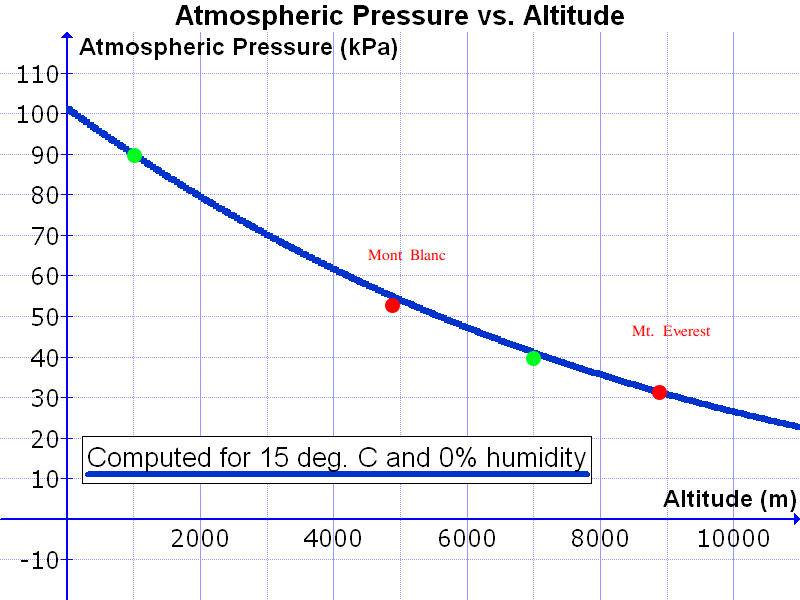
\includegraphics{Atmospheric_Pressure_vs._Altitude.png}
\caption{Atmospheric pressure versus altitude (wikipedia). Green points
represent our measurements, red points represent
interpolation/extrapolation.}
\end{figure}

    \hypertarget{discount-curve-interpolation}{%
\subsection{Discount curve
interpolation}\label{discount-curve-interpolation}}

Now we can come back to finance and using what we have just learnt try
to write a function which interpolates some given discount factors.

Needed data: * a list of pillars dates specifying the value dates of the
given discount factors, \(t_0,...,t_{n-1}\) * a list of given discount
factors, \(D(t_0),...,D(t_{n-1})\) * a pricing date (`today' date) which
corresponds to \(t=0\)

The input argument to the function will be the value date at which we
want to interpolate the discount factor.

Since the discount factor can be expresses as \(D=e^{-r(T-t)}\) the
function will use a log-linear interpolation to return the value we are
looking for.

\[D(t) = \mathrm{exp}\Big( (1-w)\cdot \mathrm{ln}(D(t_i)) + w\cdot \mathrm{ln}(D(t_{i+1}))\Big);\;\;\;w=\frac{t-t_i}{t_{i+1}-t_i}\]

where \(i\) is such that \(t_i \le t \le t_{i+1}\). More technically we
can say that we are doing a linear interpolation over time in the log
space:

\[d(t_i):=\mathrm{ln}(D(t_i))\]

\[d(t) = (1-w)d(t_i) + wd(t_{i+1});\;\;\;w=\frac{t-t_i}{t_{i+1}-t_i}\]

\[D(t) = \mathrm{exp}(d(t))\]

where \(i\) is such that \(t_i \le t \le t_{i+1}\)

Instead of reinventing the wheel and perform the interpolation with our
own code, we'll use the function \texttt{interp} provided by the Python
module \texttt{numpy}. So first let's try it with some simple examples:

    \begin{Verbatim}[commandchars=\\\{\}]
{\color{incolor}In [{\color{incolor}8}]:} \PY{c+c1}{\PYZsh{} let\PYZsq{}s assume we have a list \PYZsq{}xp\PYZsq{} of x-axis coordinates,}
        \PY{c+c1}{\PYZsh{} and the corresponding values \PYZsq{}fp\PYZsq{} of a function evaluated }
        \PY{c+c1}{\PYZsh{} at those x coordinates.}
        \PY{n}{xp} \PY{o}{=} \PY{p}{[}\PY{l+m+mi}{1}\PY{p}{,} \PY{l+m+mi}{2}\PY{p}{,} \PY{l+m+mi}{3}\PY{p}{]}
        \PY{n}{fp} \PY{o}{=} \PY{p}{[}\PY{l+m+mf}{0.3}\PY{p}{,} \PY{l+m+mf}{0.4}\PY{p}{,} \PY{l+m+mf}{0.6}\PY{p}{]}
        
        \PY{c+c1}{\PYZsh{} let\PYZsq{}s see what this looks like when plotted on a graph}
        \PY{c+c1}{\PYZsh{} we briefly introduce here the matplotlib module}
        \PY{c+c1}{\PYZsh{} the keyword as allows to give shorter names to modules}
        \PY{k+kn}{from} \PY{n+nn}{matplotlib} \PY{k}{import} \PY{n}{pyplot} \PY{k}{as} \PY{n}{plt}
        \PY{n}{plt}\PY{o}{.}\PY{n}{plot}\PY{p}{(}\PY{n}{xp}\PY{p}{,} \PY{n}{fp}\PY{p}{,} \PY{n}{marker}\PY{o}{=}\PY{l+s+s1}{\PYZsq{}}\PY{l+s+s1}{o}\PY{l+s+s1}{\PYZsq{}}\PY{p}{)}
        \PY{n}{plt}\PY{o}{.}\PY{n}{grid}\PY{p}{(}\PY{k+kc}{True}\PY{p}{)}
        \PY{n}{plt}\PY{o}{.}\PY{n}{show}\PY{p}{(}\PY{p}{)}
\end{Verbatim}

    \begin{center}
    \adjustimage{max size={0.9\linewidth}{0.9\paperheight}}{lecture_3_files/lecture_3_10_0.png}
    \end{center}
    { \hspace*{\fill} \\}
    
    \begin{Verbatim}[commandchars=\\\{\}]
{\color{incolor}In [{\color{incolor}9}]:} \PY{c+c1}{\PYZsh{} the numpy.interp function linearly interpolates these points to }
        \PY{c+c1}{\PYZsh{} estimate the value of f at other x coordinates. }
        \PY{c+c1}{\PYZsh{} For example, say we want to interpolate the points at x = 2.5::}
        \PY{k+kn}{import} \PY{n+nn}{numpy} \PY{k}{as} \PY{n+nn}{np}
        \PY{n}{np}\PY{o}{.}\PY{n}{interp}\PY{p}{(}\PY{l+m+mf}{2.5}\PY{p}{,} \PY{n}{xp}\PY{p}{,} \PY{n}{fp}\PY{p}{)}
\end{Verbatim}

\begin{Verbatim}[commandchars=\\\{\}]
{\color{outcolor}Out[{\color{outcolor}9}]:} 0.5
\end{Verbatim}
            
    \begin{Verbatim}[commandchars=\\\{\}]
{\color{incolor}In [{\color{incolor}10}]:} \PY{c+c1}{\PYZsh{} let\PYZsq{}s see what this looks like when plotted on a graph}
         
         \PY{k+kn}{from} \PY{n+nn}{matplotlib} \PY{k}{import} \PY{n}{pyplot} \PY{k}{as} \PY{n}{plt}
         \PY{n}{plt}\PY{o}{.}\PY{n}{plot}\PY{p}{(}\PY{n}{xp}\PY{p}{,} \PY{n}{fp}\PY{p}{,} \PY{n}{marker}\PY{o}{=}\PY{l+s+s1}{\PYZsq{}}\PY{l+s+s1}{o}\PY{l+s+s1}{\PYZsq{}}\PY{p}{)}
         \PY{n}{plt}\PY{o}{.}\PY{n}{grid}\PY{p}{(}\PY{k+kc}{True}\PY{p}{)}
         \PY{n}{plt}\PY{o}{.}\PY{n}{plot}\PY{p}{(}\PY{l+m+mf}{2.5}\PY{p}{,} \PY{n}{np}\PY{o}{.}\PY{n}{interp}\PY{p}{(}\PY{l+m+mf}{2.5}\PY{p}{,} \PY{n}{xp}\PY{p}{,} \PY{n}{fp}\PY{p}{)}\PY{p}{,} \PY{n}{marker}\PY{o}{=}\PY{l+s+s1}{\PYZsq{}}\PY{l+s+s1}{X}\PY{l+s+s1}{\PYZsq{}}\PY{p}{)}
         \PY{n}{plt}\PY{o}{.}\PY{n}{show}\PY{p}{(}\PY{p}{)}
\end{Verbatim}

    \begin{center}
    \adjustimage{max size={0.9\linewidth}{0.9\paperheight}}{lecture_3_files/lecture_3_12_0.png}
    \end{center}
    { \hspace*{\fill} \\}
    
    \hypertarget{interlude}{%
\subsubsection{Interlude}\label{interlude}}

How to learn about a given function ? Use the \texttt{help} keyword !

    \begin{Verbatim}[commandchars=\\\{\}]
{\color{incolor}In [{\color{incolor}11}]:} \PY{n}{help}\PY{p}{(}\PY{n}{np}\PY{o}{.}\PY{n}{interp}\PY{p}{)}
\end{Verbatim}

    \begin{Verbatim}[commandchars=\\\{\}]
Help on function interp in module numpy:

interp(x, xp, fp, left=None, right=None, period=None)
    One-dimensional linear interpolation.
    
    Returns the one-dimensional piecewise linear interpolant to a function
    with given discrete data points (`xp`, `fp`), evaluated at `x`.
    
    Parameters
    ----------
    x : array\_like
        The x-coordinates at which to evaluate the interpolated values.
    
    xp : 1-D sequence of floats
        The x-coordinates of the data points, must be increasing if argument
        `period` is not specified. Otherwise, `xp` is internally sorted after
        normalizing the periodic boundaries with ``xp = xp \% period``.
    
    fp : 1-D sequence of float or complex
        The y-coordinates of the data points, same length as `xp`.
    
    left : optional float or complex corresponding to fp
        Value to return for `x < xp[0]`, default is `fp[0]`.
    
    right : optional float or complex corresponding to fp
        Value to return for `x > xp[-1]`, default is `fp[-1]`.
    
    period : None or float, optional
        A period for the x-coordinates. This parameter allows the proper
        interpolation of angular x-coordinates. Parameters `left` and `right`
        are ignored if `period` is specified.
    
        .. versionadded:: 1.10.0
    
    Returns
    -------
    y : float or complex (corresponding to fp) or ndarray
        The interpolated values, same shape as `x`.
    
    Raises
    ------
    ValueError
        If `xp` and `fp` have different length
        If `xp` or `fp` are not 1-D sequences
        If `period == 0`
    
    Notes
    -----
    Does not check that the x-coordinate sequence `xp` is increasing.
    If `xp` is not increasing, the results are nonsense.
    A simple check for increasing is::
    
        np.all(np.diff(xp) > 0)
    
    Examples
    --------
    >>> xp = [1, 2, 3]
    >>> fp = [3, 2, 0]
    >>> np.interp(2.5, xp, fp)
    1.0
    >>> np.interp([0, 1, 1.5, 2.72, 3.14], xp, fp)
    array([ 3. ,  3. ,  2.5 ,  0.56,  0. ])
    >>> UNDEF = -99.0
    >>> np.interp(3.14, xp, fp, right=UNDEF)
    -99.0
    
    Plot an interpolant to the sine function:
    
    >>> x = np.linspace(0, 2*np.pi, 10)
    >>> y = np.sin(x)
    >>> xvals = np.linspace(0, 2*np.pi, 50)
    >>> yinterp = np.interp(xvals, x, y)
    >>> import matplotlib.pyplot as plt
    >>> plt.plot(x, y, 'o')
    [<matplotlib.lines.Line2D object at 0x{\ldots}>]
    >>> plt.plot(xvals, yinterp, '-x')
    [<matplotlib.lines.Line2D object at 0x{\ldots}>]
    >>> plt.show()
    
    Interpolation with periodic x-coordinates:
    
    >>> x = [-180, -170, -185, 185, -10, -5, 0, 365]
    >>> xp = [190, -190, 350, -350]
    >>> fp = [5, 10, 3, 4]
    >>> np.interp(x, xp, fp, period=360)
    array([7.5, 5., 8.75, 6.25, 3., 3.25, 3.5, 3.75])
    
    Complex interpolation:
    
    >>> x = [1.5, 4.0]
    >>> xp = [2,3,5]
    >>> fp = [1.0j, 0, 2+3j]
    >>> np.interp(x, xp, fp)
    array([ 0.+1.j ,  1.+1.5j])


    \end{Verbatim}

    \hypertarget{now-back-to-our-discount-factor-function-df.}{%
\subsubsection{Now back to our discount factor function
df.}\label{now-back-to-our-discount-factor-function-df.}}

    \begin{Verbatim}[commandchars=\\\{\}]
{\color{incolor}In [{\color{incolor}12}]:} \PY{c+c1}{\PYZsh{} import modules and objects that we need}
         \PY{k+kn}{from} \PY{n+nn}{datetime} \PY{k}{import} \PY{n}{date}
         \PY{k+kn}{import} \PY{n+nn}{numpy}\PY{o}{,} \PY{n+nn}{math}
         \PY{k+kn}{from} \PY{n+nn}{matplotlib} \PY{k}{import} \PY{n}{pyplot} \PY{k}{as} \PY{n}{plt}
         \PY{k+kn}{import} \PY{n+nn}{matplotlib}\PY{n+nn}{.}\PY{n+nn}{dates} \PY{k}{as} \PY{n+nn}{mdates} 
         \PY{c+c1}{\PYZsh{} with this notation we tell python to use mdates as an alias }
         \PY{c+c1}{\PYZsh{} for matplotlib.dates, I told you I\PYZsq{}m lazy...}
         
         \PY{c+c1}{\PYZsh{} define the input data}
         \PY{n}{today\PYZus{}date} \PY{o}{=} \PY{n}{date}\PY{p}{(}\PY{l+m+mi}{2019}\PY{p}{,} \PY{l+m+mi}{10}\PY{p}{,} \PY{l+m+mi}{1}\PY{p}{)}
         
         \PY{n}{pillar\PYZus{}dates} \PY{o}{=} \PY{p}{[}\PY{n}{date}\PY{p}{(}\PY{l+m+mi}{2019}\PY{p}{,} \PY{l+m+mi}{10}\PY{p}{,} \PY{l+m+mi}{1}\PY{p}{)}\PY{p}{,} \PY{n}{date}\PY{p}{(}\PY{l+m+mi}{2020}\PY{p}{,} \PY{l+m+mi}{10}\PY{p}{,} \PY{l+m+mi}{1}\PY{p}{)}\PY{p}{,} \PY{n}{date}\PY{p}{(}\PY{l+m+mi}{2021}\PY{p}{,} \PY{l+m+mi}{10}\PY{p}{,} \PY{l+m+mi}{1}\PY{p}{)}\PY{p}{]}
         \PY{n}{discount\PYZus{}factors} \PY{o}{=} \PY{p}{[}\PY{l+m+mf}{1.0}\PY{p}{,} \PY{l+m+mf}{0.97}\PY{p}{,} \PY{l+m+mf}{0.72}\PY{p}{]}
         
         \PY{c+c1}{\PYZsh{} let\PYZsq{}s see what this looks like when plotted on a graph}
         \PY{c+c1}{\PYZsh{} here a more complicated usage of matplotlib to}
         \PY{c+c1}{\PYZsh{} get a nicer plot}
         \PY{n}{plt}\PY{o}{.}\PY{n}{plot}\PY{p}{(}\PY{n}{pillar\PYZus{}dates}\PY{p}{,} \PY{n}{discount\PYZus{}factors}\PY{p}{,} \PY{n}{marker}\PY{o}{=}\PY{l+s+s1}{\PYZsq{}}\PY{l+s+s1}{o}\PY{l+s+s1}{\PYZsq{}}\PY{p}{)}
         \PY{n}{plt}\PY{o}{.}\PY{n}{gca}\PY{p}{(}\PY{p}{)}\PY{o}{.}\PY{n}{xaxis}\PY{o}{.}\PY{n}{set\PYZus{}major\PYZus{}formatter}\PY{p}{(}\PY{n}{mdates}\PY{o}{.}\PY{n}{DateFormatter}\PY{p}{(}\PY{l+s+s1}{\PYZsq{}}\PY{l+s+s1}{\PYZpc{}}\PY{l+s+s1}{m/}\PY{l+s+si}{\PYZpc{}d}\PY{l+s+s1}{/}\PY{l+s+s1}{\PYZpc{}}\PY{l+s+s1}{Y}\PY{l+s+s1}{\PYZsq{}}\PY{p}{)}\PY{p}{)}
         \PY{n}{plt}\PY{o}{.}\PY{n}{gca}\PY{p}{(}\PY{p}{)}\PY{o}{.}\PY{n}{xaxis}\PY{o}{.}\PY{n}{set\PYZus{}major\PYZus{}locator}\PY{p}{(}\PY{n}{mdates}\PY{o}{.}\PY{n}{YearLocator}\PY{p}{(}\PY{p}{)}\PY{p}{)}
         \PY{n}{plt}\PY{o}{.}\PY{n}{grid}\PY{p}{(}\PY{k+kc}{True}\PY{p}{)}
         \PY{n}{plt}\PY{o}{.}\PY{n}{show}\PY{p}{(}\PY{p}{)}
         
         \PY{c+c1}{\PYZsh{} define the df function}
         \PY{k}{def} \PY{n+nf}{df}\PY{p}{(}\PY{n}{d}\PY{p}{)}\PY{p}{:}
             \PY{c+c1}{\PYZsh{} first thing we need to do is to apply the logarithm function }
             \PY{c+c1}{\PYZsh{} to the discount factors since we are doing log-linear and}
             \PY{c+c1}{\PYZsh{} not just linear interpolation}
             \PY{n}{log\PYZus{}discount\PYZus{}factors} \PY{o}{=} \PY{p}{[}\PY{p}{]}
             \PY{k}{for} \PY{n}{discount\PYZus{}factor} \PY{o+ow}{in} \PY{n}{discount\PYZus{}factors}\PY{p}{:}
                 \PY{n}{log\PYZus{}discount\PYZus{}factors}\PY{o}{.}\PY{n}{append}\PY{p}{(}\PY{n}{math}\PY{o}{.}\PY{n}{log}\PY{p}{(}\PY{n}{discount\PYZus{}factor}\PY{p}{)}\PY{p}{)}
             
             \PY{c+c1}{\PYZsh{} perform the linear interpolation of the log discount factors}
             \PY{n}{interpolated\PYZus{}log\PYZus{}discount\PYZus{}factor} \PY{o}{=} \PYZbs{}
                 \PY{n}{numpy}\PY{o}{.}\PY{n}{interp}\PY{p}{(}\PY{n}{d}\PY{p}{,} \PY{n}{pillar\PYZus{}dates}\PY{p}{,} \PY{n}{log\PYZus{}discount\PYZus{}factors}\PY{p}{)}
             
             \PY{c+c1}{\PYZsh{} return the interpolated discount factor}
             \PY{k}{return} \PY{n}{math}\PY{o}{.}\PY{n}{exp}\PY{p}{(}\PY{n}{interpolated\PYZus{}log\PYZus{}discount\PYZus{}factor}\PY{p}{)}
\end{Verbatim}

    \begin{center}
    \adjustimage{max size={0.9\linewidth}{0.9\paperheight}}{lecture_3_files/lecture_3_16_0.png}
    \end{center}
    { \hspace*{\fill} \\}
    
    This is almost OK, \textbf{but it won't work} because
\texttt{numpy.interp} only accepts numbers/lists of numbers as arguments
i.e.~it doesn't automatically convert or interpret dates as numbers in
any way, so it doesn't know how to interpolate them. So we need to do
the conversion ourselves before passing the data into the
\texttt{numpy.interp} function.

    \begin{Verbatim}[commandchars=\\\{\}]
{\color{incolor}In [{\color{incolor}13}]:} \PY{k}{def} \PY{n+nf}{df}\PY{p}{(}\PY{n}{d}\PY{p}{)}\PY{p}{:}
             \PY{c+c1}{\PYZsh{} first thing we need to do is to apply the logarithm function}
             \PY{c+c1}{\PYZsh{} to the discount factors since we are doing log-linear and}
             \PY{c+c1}{\PYZsh{} not just linear interpolation}
             \PY{n}{log\PYZus{}discount\PYZus{}factors} \PY{o}{=} \PY{p}{[}\PY{p}{]}
             \PY{k}{for} \PY{n}{discount\PYZus{}factor} \PY{o+ow}{in} \PY{n}{discount\PYZus{}factors}\PY{p}{:}
                 \PY{n}{log\PYZus{}discount\PYZus{}factors}\PY{o}{.}\PY{n}{append}\PY{p}{(}\PY{n}{math}\PY{o}{.}\PY{n}{log}\PY{p}{(}\PY{n}{discount\PYZus{}factor}\PY{p}{)}\PY{p}{)}
             
             \PY{c+c1}{\PYZsh{} convert the pillar dates to pillar \PYZsq{}days\PYZsq{}}
             \PY{c+c1}{\PYZsh{} i.e. number of days from today}
             \PY{c+c1}{\PYZsh{} to write shorter code we can use this NEW notation}
             \PY{c+c1}{\PYZsh{} which condenses for and list creation in one line}
             \PY{n}{pillar\PYZus{}days} \PY{o}{=} \PYZbs{}
                 \PY{p}{[}\PY{p}{(}\PY{n}{pillar\PYZus{}date} \PY{o}{\PYZhy{}} \PY{n}{today\PYZus{}date}\PY{p}{)}\PY{o}{.}\PY{n}{days} \PY{k}{for} \PY{n}{pillar\PYZus{}date} \PY{o+ow}{in} \PY{n}{pillar\PYZus{}dates}\PY{p}{]}
             
             \PY{c+c1}{\PYZsh{} obviously we need to do the same to the value date}
             \PY{c+c1}{\PYZsh{} argument of the df function}
             \PY{n}{d\PYZus{}days} \PY{o}{=} \PY{p}{(}\PY{n}{d} \PY{o}{\PYZhy{}} \PY{n}{today\PYZus{}date}\PY{p}{)}\PY{o}{.}\PY{n}{days}
             
             \PY{c+c1}{\PYZsh{} perform the linear interpolation of the log discount factors}
             \PY{n}{interpolated\PYZus{}log\PYZus{}discount\PYZus{}factor} \PY{o}{=} \PYZbs{}
                 \PY{n}{numpy}\PY{o}{.}\PY{n}{interp}\PY{p}{(}\PY{n}{d\PYZus{}days}\PY{p}{,} \PY{n}{pillar\PYZus{}days}\PY{p}{,} \PY{n}{log\PYZus{}discount\PYZus{}factors}\PY{p}{)}
             
             \PY{c+c1}{\PYZsh{} return the interpolated discount factor}
             \PY{k}{return} \PY{n}{math}\PY{o}{.}\PY{n}{exp}\PY{p}{(}\PY{n}{interpolated\PYZus{}log\PYZus{}discount\PYZus{}factor}\PY{p}{)}
\end{Verbatim}

    \begin{Verbatim}[commandchars=\\\{\}]
{\color{incolor}In [{\color{incolor}18}]:} \PY{c+c1}{\PYZsh{} now we can use the df function to get discount factors}
         \PY{c+c1}{\PYZsh{} on value dates between the given pillar dates}
         \PY{n}{d0} \PY{o}{=} \PY{n}{date}\PY{p}{(}\PY{l+m+mi}{2020}\PY{p}{,} \PY{l+m+mi}{1}\PY{p}{,} \PY{l+m+mi}{1}\PY{p}{)}
         \PY{n}{df0} \PY{o}{=} \PY{n}{df}\PY{p}{(}\PY{n}{d0}\PY{p}{)}
         \PY{n+nb}{print} \PY{p}{(}\PY{n}{df0}\PY{p}{)}
\end{Verbatim}

    \begin{Verbatim}[commandchars=\\\{\}]
0.9923728228571693

    \end{Verbatim}

    \begin{Verbatim}[commandchars=\\\{\}]
{\color{incolor}In [{\color{incolor}15}]:} \PY{n}{d1} \PY{o}{=} \PY{n}{date}\PY{p}{(}\PY{l+m+mi}{2021}\PY{p}{,} \PY{l+m+mi}{1}\PY{p}{,} \PY{l+m+mi}{1}\PY{p}{)}
         \PY{n}{df1} \PY{o}{=} \PY{n}{df}\PY{p}{(}\PY{n}{d1}\PY{p}{)}
         \PY{n+nb}{print} \PY{p}{(}\PY{n}{df1}\PY{p}{)}
\end{Verbatim}

    \begin{Verbatim}[commandchars=\\\{\}]
0.8997999273630835

    \end{Verbatim}

    \begin{Verbatim}[commandchars=\\\{\}]
{\color{incolor}In [{\color{incolor}19}]:} \PY{c+c1}{\PYZsh{} let\PYZsq{}s see what these look like when plotted on a semi-log graph}
         
         \PY{k+kn}{from} \PY{n+nn}{matplotlib} \PY{k}{import} \PY{n}{pyplot} \PY{k}{as} \PY{n}{plt}
         \PY{k+kn}{import} \PY{n+nn}{matplotlib}\PY{n+nn}{.}\PY{n+nn}{dates} \PY{k}{as} \PY{n+nn}{mdates}
         \PY{n}{plt}\PY{o}{.}\PY{n}{semilogy}\PY{p}{(}\PY{n}{pillar\PYZus{}dates}\PY{p}{,} \PY{n}{discount\PYZus{}factors}\PY{p}{,} \PY{n}{marker}\PY{o}{=}\PY{l+s+s1}{\PYZsq{}}\PY{l+s+s1}{o}\PY{l+s+s1}{\PYZsq{}}\PY{p}{)}
         \PY{n}{plt}\PY{o}{.}\PY{n}{semilogy}\PY{p}{(}\PY{n}{d0}\PY{p}{,}\PY{n}{df0} \PY{p}{,} \PY{n}{marker}\PY{o}{=}\PY{l+s+s1}{\PYZsq{}}\PY{l+s+s1}{X}\PY{l+s+s1}{\PYZsq{}}\PY{p}{)}
         \PY{n}{plt}\PY{o}{.}\PY{n}{semilogy}\PY{p}{(}\PY{n}{d1}\PY{p}{,}\PY{n}{df1} \PY{p}{,} \PY{n}{marker}\PY{o}{=}\PY{l+s+s1}{\PYZsq{}}\PY{l+s+s1}{X}\PY{l+s+s1}{\PYZsq{}}\PY{p}{)}
         \PY{n}{plt}\PY{o}{.}\PY{n}{gca}\PY{p}{(}\PY{p}{)}\PY{o}{.}\PY{n}{xaxis}\PY{o}{.}\PY{n}{set\PYZus{}major\PYZus{}formatter}\PY{p}{(}\PY{n}{mdates}\PY{o}{.}\PY{n}{DateFormatter}\PY{p}{(}\PY{l+s+s1}{\PYZsq{}}\PY{l+s+s1}{\PYZpc{}}\PY{l+s+s1}{m/}\PY{l+s+si}{\PYZpc{}d}\PY{l+s+s1}{/}\PY{l+s+s1}{\PYZpc{}}\PY{l+s+s1}{Y}\PY{l+s+s1}{\PYZsq{}}\PY{p}{)}\PY{p}{)}
         \PY{n}{plt}\PY{o}{.}\PY{n}{gca}\PY{p}{(}\PY{p}{)}\PY{o}{.}\PY{n}{xaxis}\PY{o}{.}\PY{n}{set\PYZus{}major\PYZus{}locator}\PY{p}{(}\PY{n}{mdates}\PY{o}{.}\PY{n}{YearLocator}\PY{p}{(}\PY{p}{)}\PY{p}{)}
         \PY{n}{plt}\PY{o}{.}\PY{n}{grid}\PY{p}{(}\PY{k+kc}{True}\PY{p}{)}
         \PY{n}{plt}\PY{o}{.}\PY{n}{show}\PY{p}{(}\PY{p}{)}
\end{Verbatim}

    \begin{center}
    \adjustimage{max size={0.9\linewidth}{0.9\paperheight}}{lecture_3_files/lecture_3_21_0.png}
    \end{center}
    { \hspace*{\fill} \\}
    
    \begin{Verbatim}[commandchars=\\\{\}]
{\color{incolor}In [{\color{incolor}20}]:} \PY{c+c1}{\PYZsh{} let\PYZsq{}s see what these look like when plotted on a linear graph}
         
         \PY{k+kn}{from} \PY{n+nn}{matplotlib} \PY{k}{import} \PY{n}{pyplot} \PY{k}{as} \PY{n}{plt}
         \PY{k+kn}{import} \PY{n+nn}{matplotlib}\PY{n+nn}{.}\PY{n+nn}{dates} \PY{k}{as} \PY{n+nn}{mdates}
         \PY{n}{plt}\PY{o}{.}\PY{n}{plot}\PY{p}{(}\PY{n}{pillar\PYZus{}dates}\PY{p}{,} \PY{n}{discount\PYZus{}factors}\PY{p}{,} \PY{n}{marker}\PY{o}{=}\PY{l+s+s1}{\PYZsq{}}\PY{l+s+s1}{o}\PY{l+s+s1}{\PYZsq{}}\PY{p}{)}
         \PY{n}{plt}\PY{o}{.}\PY{n}{plot}\PY{p}{(}\PY{n}{d0}\PY{p}{,}\PY{n}{df0} \PY{p}{,} \PY{n}{marker}\PY{o}{=}\PY{l+s+s1}{\PYZsq{}}\PY{l+s+s1}{X}\PY{l+s+s1}{\PYZsq{}}\PY{p}{)}
         \PY{n}{plt}\PY{o}{.}\PY{n}{plot}\PY{p}{(}\PY{n}{d1}\PY{p}{,}\PY{n}{df1} \PY{p}{,} \PY{n}{marker}\PY{o}{=}\PY{l+s+s1}{\PYZsq{}}\PY{l+s+s1}{X}\PY{l+s+s1}{\PYZsq{}}\PY{p}{)}
         \PY{n}{plt}\PY{o}{.}\PY{n}{gca}\PY{p}{(}\PY{p}{)}\PY{o}{.}\PY{n}{xaxis}\PY{o}{.}\PY{n}{set\PYZus{}major\PYZus{}formatter}\PY{p}{(}\PY{n}{mdates}\PY{o}{.}\PY{n}{DateFormatter}\PY{p}{(}\PY{l+s+s1}{\PYZsq{}}\PY{l+s+s1}{\PYZpc{}}\PY{l+s+s1}{m/}\PY{l+s+si}{\PYZpc{}d}\PY{l+s+s1}{/}\PY{l+s+s1}{\PYZpc{}}\PY{l+s+s1}{Y}\PY{l+s+s1}{\PYZsq{}}\PY{p}{)}\PY{p}{)}
         \PY{n}{plt}\PY{o}{.}\PY{n}{gca}\PY{p}{(}\PY{p}{)}\PY{o}{.}\PY{n}{xaxis}\PY{o}{.}\PY{n}{set\PYZus{}major\PYZus{}locator}\PY{p}{(}\PY{n}{mdates}\PY{o}{.}\PY{n}{YearLocator}\PY{p}{(}\PY{p}{)}\PY{p}{)}
         \PY{n}{plt}\PY{o}{.}\PY{n}{grid}\PY{p}{(}\PY{k+kc}{True}\PY{p}{)}
         \PY{n}{plt}\PY{o}{.}\PY{n}{show}\PY{p}{(}\PY{p}{)}
\end{Verbatim}

    \begin{center}
    \adjustimage{max size={0.9\linewidth}{0.9\paperheight}}{lecture_3_files/lecture_3_22_0.png}
    \end{center}
    { \hspace*{\fill} \\}
    
    \hypertarget{exercises}{%
\subsection{Exercises}\label{exercises}}

\hypertarget{exercise-3.1}{%
\subsubsection{Exercise 3.1}\label{exercise-3.1}}

Take the code for the Black-Scholes formula from Exercise 2.3 and wrap
it in a function. Then, use this function to calculate the prices of
calls with various strikes, using the following data.

\begin{Shaded}
\begin{Highlighting}[]
\NormalTok{S_t }\OperatorTok{=} \DecValTok{800}
\CommentTok{# strikes expressed as % of spot price}
\NormalTok{moneyness }\OperatorTok{=}\NormalTok{ [ }\FloatTok{0.5}\NormalTok{, }\FloatTok{0.75}\NormalTok{, }\FloatTok{0.825}\NormalTok{, }\FloatTok{1.0}\NormalTok{, }\FloatTok{1.125}\NormalTok{, }\FloatTok{1.25}\NormalTok{, }\FloatTok{1.5}\NormalTok{ ]   }
\NormalTok{vol }\OperatorTok{=} \FloatTok{0.3}
\NormalTok{ttm }\OperatorTok{=} \FloatTok{0.75}
\NormalTok{r }\OperatorTok{=} \FloatTok{0.005}
\end{Highlighting}
\end{Shaded}

The output should be a dictionary mapping strikes to call prices.

\hypertarget{exercise-3.2}{%
\subsubsection{Exercise 3.2}\label{exercise-3.2}}

Python has a useful command called \texttt{assert} which can be used for
checking that a given condition is satisfied, and raising an error if
the condition is not satisfied.

The following line does not cause an error, in fact it does nothing

\begin{Shaded}
\begin{Highlighting}[]
\ControlFlowTok{assert} \DecValTok{1} \OperatorTok{<} \DecValTok{2}
\end{Highlighting}
\end{Shaded}

This causes an error

\begin{Shaded}
\begin{Highlighting}[]
\ControlFlowTok{assert} \DecValTok{1} \OperatorTok{>} \DecValTok{2}
\end{Highlighting}
\end{Shaded}

\texttt{assert} can take a second parameter with a message to display in case of failure:

\begin{Shaded}
\begin{Highlighting}[]
\ControlFlowTok{assert} \DecValTok{1} \OperatorTok{>} \DecValTok{2}, ``Two is bigger than one''
\end{Highlighting}
\end{Shaded}

Take the \texttt{df} function from this lesson and modify it by adding some
assertions to check that:
\begin{itemize}
\item the pillar date list contains at least 2 elements
\item the pillar date list is the same length as the discount factor list
\item the first pillar date is equal to the today date
\item the value date argument 'd' is greater or equal to the first pillar date and also less than or equal to the last pillar date
\end{itemize}

Then try using the function with some invalid data to make sure that
your assertions are correctly checking the desired conditions.

\hypertarget{exercise-3.3}{%
\subsubsection{Exercise 3.3}\label{exercise-3.3}}

Python has a module called \texttt{matplotlib} which can be used for
plotting graphs and charts. In particular, we can use a sub-module
called \texttt{pyplot} which provides slightly easier-to-use interface
for plotting interactively.

\begin{Shaded}
\begin{Highlighting}[]
\ImportTok{from}\NormalTok{ matplotlib }\ImportTok{import}\NormalTok{ pyplot}

\CommentTok{# plot some data}
\NormalTok{pyplot.plot(}
\NormalTok{    [}\DecValTok{1}\NormalTok{, }\DecValTok{2}\NormalTok{, }\DecValTok{3}\NormalTok{],   }\CommentTok{# x-axis coordinates}
\NormalTok{    [}\DecValTok{5}\NormalTok{, }\DecValTok{3}\NormalTok{, }\DecValTok{10}\NormalTok{],  }\CommentTok{# y-axis coordinates}
\NormalTok{    marker}\OperatorTok{=}\StringTok{'o'}   \CommentTok{# we want the points to be marked with circles}
\NormalTok{)}
\end{Highlighting}
\end{Shaded}

Use this function to plot the call prices from exercise 3.1. Remember to
use \texttt{help} and \texttt{dir} to have some help (or to look in
Google ;-)).

    \hypertarget{advanced-hint}{%
\subsection{Advanced hint}\label{advanced-hint}}

Interpolation using \texttt{scipy.interpolate}:
https://docs.scipy.org/doc/scipy-0.15.1/reference/interpolate.html\#module-scipy.interpolate


    % Add a bibliography block to the postdoc
    
    
    
    \end{document}
